% Chapter 3 — Methodology

\chapter{Methodology}
\label{Chapter3}

%----------------------------------------------------------------------------------------

\section{Overview}

This chapter describes the complete implementation of MIGA from the paper specification, documents every decision made where the paper is ambiguous or silent, and presents the novel extensions introduced in this thesis: IPW-$F_r$ for MNAR bias correction (C6, Section~\ref{sec:ipw_implementation}) and the synthetic dimension experiment methodology (C5, Section~\ref{sec:synthetic_dim_methods}). The formal $F_r$--RMSE orthogonality result (Chapter~\ref{Chapter2}, Propositions~\ref{prop:rmse_implies_fr}--\ref{prop:fr_implies_rmse}) provides the theoretical framework within which all contributions are situated.

All code is implemented in Python 3.12 using NumPy, SciPy, and scikit-learn. The implementation is structured as a Python package (\texttt{miga/}) with the modules described in Table~\ref{tab:modules}.

\begin{table}[h]
\caption{Python package module structure.}
\label{tab:modules}
\centering
\begin{tabular}{lp{9.5cm}}
\toprule
\textbf{Module} & \textbf{Responsibility} \\
\midrule
\texttt{miga/statistics.py} & Statistical primitives: \texttt{compute\_stats}, \texttt{compute\_kurtosis}, \texttt{ledoit\_wolf\_cov} \\
\texttt{miga/fitness.py}    & \texttt{FitnessEvaluator}: pre-computes $X_A$ statistics, evaluates $F_r$ (with optional IPW weighting) \\
\texttt{miga/operators.py}  & \texttt{initialize\_population}, \texttt{mutate}, \texttt{crossover}, \texttt{diversity} \\
\texttt{miga/core.py}       & \texttt{MIGA}: top-level estimator, orchestrates $Q$ runs \\
\texttt{miga/data\_utils.py}& Dataset loaders, \texttt{apply\_mar}, \texttt{apply\_mnar}, \texttt{auto\_generators} \\
\bottomrule
\end{tabular}
\end{table}

%----------------------------------------------------------------------------------------

\section{Reimplementation of MIGA (C1)}

\subsection{Population Representation}

Each individual in the genetic algorithm population represents a complete candidate imputation for all missing cells in the dataset. If the dataset has $k$ missing cells (across all rows in $X_C$), an individual is a vector of $k$ real numbers. The mapping between positions in this vector and (row, column) locations in the dataset is stored as a list \texttt{missing\_index} of (local\_row, col) pairs, constructed once before the GA begins.

This flat vector representation is efficient: fitness evaluation requires only reassembling $X_C$ from the current individual and computing the three statistical distances. The population is stored as a 2D array of shape $(l, k)$.

\subsection{Fitness Evaluation}

The fitness function $F_r$ is evaluated by \texttt{FitnessEvaluator}, which pre-computes all $X_A$ statistics at initialisation (mean, covariance, skewness, and optionally kurtosis) and evaluates each candidate $X_C$ efficiently. Feature scaling is applied before all computations (\S\ref{sec:scaling}).

The three terms follow Equations 5--10 of Figueroa-Garc\'ia et al. (2023) \cite{FigueroaGarcia2023}:

\textbf{$d_{\text{means}}$ --- Standardised mean distance:}
\begin{equation}
    d_{\text{means}} = D_r\!\left(\tilde{x}_A,\, \tilde{x}_C\right), \quad \tilde{x} = \frac{\bar{x}}{S_p}
\end{equation}
where $S_p$ is the pooled standard deviation vector:
\begin{equation}
    S_{p,j}^2 = \frac{\text{diag}(S_A)_j \cdot \nu_A + \text{diag}(S_C)_j \cdot \nu_C}{\nu_A + \nu_C}
\end{equation}
with $\nu_A = n_A - 1$, $\nu_C = n_C - 1$.

\textbf{$d_{\text{cov}}$ --- Relative covariance distance:}
\begin{equation}
    d_{\text{cov}} = D_r\!\left(\tilde{S},\, I\right), \quad \tilde{S} = S_A^{-1/2} S_C S_A^{-1/2}
\end{equation}
$\tilde{S} = I$ if and only if $S_C = S_A$. The matrix square root is computed via eigendecomposition: $S_A^{-1/2} = V \Lambda^{-1/2} V^\top$.

\textbf{$d_{\text{skew}}$ --- Skewness distance:}
\begin{equation}
    d_{\text{skew}} = D_r\!\left(b_A,\, b_C\right)
\end{equation}
where $b_j$ is the bias-corrected sample skewness of column $j$.

All distances use the Minkowski order $r$ specified in the paper (typically $r = \infty$, the Chebyshev norm: $D_\infty(A, B) = \max_{i,j} |a_{ij} - b_{ij}|$).

\subsection{Feature Scaling}
\label{sec:scaling}

\textbf{Problem.} Wine's Proline feature has variance $\sigma^2 \approx 10^5$ while other features have $\sigma^2 \approx 1$. Without scaling, the condition number of $S_A$ is approximately $4 \times 10^7$, making $S_A^{-1/2}$ numerically meaningless and $d_{\text{cov}}(X_A, X_A) \neq 0$.

\textbf{Solution.} Before computing any statistics, divide each column of $X_A$ and $X_C$ by $\hat{\sigma}_j = \text{std}(X_A[:,j])$ (estimated from $X_A$ alone, to avoid data leakage from $X_C$). This transforms $S_A$ into a correlation matrix with eigenvalues bounded by $O(p)$.

After scaling, Wine 30\% condition number drops from $4 \times 10^7$ to 158 and $d_{\text{cov}}(X_A, X_A) = 0.000$.

\subsection{Eigenvalue Floor in Relative Covariance}

Even after feature scaling, $S_A$ can be rank-deficient when $n_A < p$. In \texttt{relative\_cov()}, eigenvalues of $S_A$ are floored at $\max(\lambda_{\max} \times 10^{-4}, 10^{-10})$ before computing $\Lambda^{-1/2}$. This bounds the condition number of $S_A^{-1/2}$ at $10^2$, preventing catastrophic noise amplification.

\subsection{Bootstrap Generators}
\label{sec:generators}

The paper specifies that generators $R_j$ are ``obtained from samples'' of the observed values of variable $j$. We interpret this as bootstrap resampling from the empirical distribution: $R_j$ draws uniformly from the set of non-missing observed values of column $j$.

For integer-valued columns, the generator returns integer samples only. This is essential for datasets with discrete features: Haberman's Nodes column has 44\% zeros, and a Gaussian generator would never generate zero. The bootstrap generator samples zeros with probability 0.44, correctly preserving the discrete marginal distribution.

\subsection{Genetic Algorithm Operators}

\textbf{Selection.} The top-$c$ individuals (lowest $F_r$) are retained as elites unchanged.

\textbf{Mutation.} Each of the $c_1$ elites produces $c_3$ mutated copies. A mutated copy is identical to its parent except that one randomly chosen component (one missing cell value) is replaced by a fresh sample from $R_j$ for the corresponding column $j$.

\textbf{Crossover.} $c_2$ crossover offspring are produced by uniform crossover of random pairs drawn from the elites. Each component of the offspring is taken from one parent with probability 0.5.

\textbf{Diversity injection.} The remaining $l - c - c_1 c_3 - 2(c_2 - 1)$ population slots are filled with fresh random individuals sampled entirely from the generators. Under the paper's default parameters ($l=200$, $c=3$, $c_1=3$, $c_2=2$, $c_3=5$), this is 180 individuals, or 90\% of the population.

\subsection{Multi-Run Strategy}

MIGA runs $Q$ independent GA instances on the same missing dataset, each with a different internal random seed. The best individual across all $Q$ runs is returned as the final imputation. \texttt{miga.generation\_history\_} stores the full convergence curve (best $F_r$ per generation) for each run, enabling convergence analysis.

%----------------------------------------------------------------------------------------

\section{Ledoit-Wolf Shrinkage Covariance (C2)}

\subsection{The Rank-Deficiency Problem}

The relative covariance term $d_{\text{cov}} = D_r(S_A^{-1/2} S_C S_A^{-1/2}, I)$ requires computing $S_A^{-1/2}$, which is undefined when $S_A$ is rank-deficient. $S_A$ becomes rank-deficient when $n_A < p$.

For Wine at 40\% missing: $n_A = 11$, $p = 13$. The sample covariance has condition number $5.7 \times 10^8$ and $d_{\text{cov}}(X_A, X_A) = 0.606$, a mathematical impossibility since $d_{\text{cov}}$ should equal zero when both arguments are the same set.

\subsection{The Ledoit-Wolf Estimator}

The Ledoit-Wolf (2004) shrinkage estimator \cite{LedoitWolf2004} replaces the sample covariance with a convex combination:

\begin{equation}
    S_{\text{LW}} = (1 - \alpha)\, S_{\text{sample}} + \alpha \cdot \frac{\text{tr}(S_{\text{sample}})}{p} \cdot I
\end{equation}

where $\alpha \in [0, 1]$ is the shrinkage coefficient chosen analytically. The target $(\text{tr}(S)/p) \cdot I$ is always positive definite, so $S_{\text{LW}}$ is positive definite for any $\alpha > 0$.

We apply the Ledoit-Wolf estimator to \textbf{both} $S_A$ and $S_C$. Applying it to $S_A$ alone would break the invariant $d_{\text{cov}}(X_A, X_A) = 0$.

\subsection{Results}

\begin{table}[h]
\caption{Wine: sample vs Ledoit-Wolf covariance at increasing missing rates.}
\label{tab:lw}
\centering
\begin{tabular}{llllll}
\toprule
\textbf{Missing} & $n_A$ & \textbf{Sample cond.} & \textbf{LW cond.} & $d_{\text{cov}}$ \textbf{sample} & $d_{\text{cov}}$ \textbf{LW} \\
\midrule
30\% & 23 & 158         & 9.1 & 0.000 \checkmark & 0.000 \checkmark \\
40\% & 11 & 570,000,000 & 8.8 & 0.606 $\times$   & 0.000 \checkmark \\
\bottomrule
\end{tabular}
\end{table}

Ledoit-Wolf restores mathematical consistency at 40\% missing. RMSE is not improved --- $n_A = 11$ is an insufficient sample size to reliably estimate the joint distribution of 13 features, regardless of the covariance estimator.

%----------------------------------------------------------------------------------------

\section{Budget-Aware Restarts with Adaptive Diversity Decay (C3)}
\label{sec:budget_aware}

\subsection{Motivation}

Standard MIGA allocates a fixed budget of $Q$ runs each of $G$ generations. However, fitness curves in practice converge within 100--300 generations on most datasets, leaving the remainder of each run idle. On Haberman, for example, the GA reaches its best $F_r$ within the first $\sim$150 generations and then stagnates, wasting 70\% of the budget.

The diversity injection mechanism fills 90\% of the population with random individuals at every generation. This is well-suited for exploration early in a run, but is counter-productive late in a run once the elite solutions have converged: fresh random individuals can only dislodge the elite by chance. At that point, more restarts with fresh populations would be more productive than continued random injection around a stagnated solution.

\subsection{Implementation}

Two components work together:

\textbf{Early stopping.} Each run tracks a stagnation counter incremented whenever the best $F_r$ fails to improve by more than $\varepsilon = 10^{-8}$. When the counter reaches the patience threshold $P$, the run terminates:

\begin{equation}
    \text{stop run if } \min_{g' \leq g} F_r(g') - F_r(g) < \varepsilon \text{ for } P \text{ consecutive generations}
\end{equation}

\textbf{Budget-aware restarts.} The total generation budget $B = Q \times G$ is fixed. Instead of exactly $Q$ runs of length $G$, the algorithm launches restarts in sequence until the budget is exhausted:

\begin{equation}
    \text{while } \sum_{\text{runs}} |\text{gen\_history}| < B: \quad \text{launch new run}
\end{equation}

Each run is capped at $\min(G,\, B - \text{gens\_used})$ generations so the total never exceeds $B$.

\textbf{Adaptive diversity decay.} Within each run, the number of random (diversity) individuals decays linearly from $n_{\text{div}}^{\max}$ (90\% of $l$) at generation 0 to $(1-\delta) \cdot n_{\text{div}}^{\max}$ at generation $G$, with $\delta = 0.7$:

\begin{equation}
    n_{\text{div}}(g) = \left\lfloor n_{\text{div}}^{\max} \cdot \left(1 - \delta \cdot \frac{g}{G-1}\right) \right\rfloor
\end{equation}

Slots freed by reduced diversity are filled with additional mutation offspring from the elite pool, progressively shifting the population from exploration to exploitation as each run matures. When early stopping triggers before full decay, the harmful late-stage exploitation phase is avoided.

Parameters: $P = 50$, $\delta = 0.7$, activated via \texttt{MIGA(early\_stopping\_patience=50, diversity\_decay=0.7)}.

\subsection{Why the Components Need Each Other}

Diversity decay alone was tested at full $G=500$ and worsened RMSE by 14--16\% on Haberman: late-stage exploitation of a stagnated run amplifies a poor local optimum. Early stopping alone gives more restarts but each run still spends its later generations doing 90\% random injection around a converged solution. Together: early stopping prevents the harmful late-decay phase, while decay ensures that the fraction of the budget spent near good solutions grows over the run's lifetime.

%----------------------------------------------------------------------------------------

\section{MNAR Evaluation Framework (C4)}

\subsection{Implementation of MNAR Mechanisms}

The paper evaluates MIGA only under MAR. We implement three MNAR mechanisms in \texttt{apply\_mnar(X, pct, mechanism)}:

\textbf{top:} For each selected feature $j$, the $n_{\text{remove}}$ rows with the highest values of $X_{:,j}$ are set missing.

\textbf{bottom:} The $n_{\text{remove}}$ rows with the lowest values are set missing.

\textbf{tails:} Half the removals come from each extreme: $\text{half} = \max(1, \lfloor n_{\text{remove}}/2 \rfloor)$, removing from both the top and bottom of the distribution.

\subsection{Why MNAR Breaks MIGA's Objective}

Under MAR, $X_A$ is a representative sample of the full population. The fitness function's goal --- make $X_C$ look like $X_A$ --- is equivalent to making $X_C$ look like the true population.

Under MNAR \texttt{top}, rows with high values of the selected features go missing, so $X_A$ contains only rows with low values for those features. The fitness function instructs the GA to match $X_C$ to this biased $X_A$. The GA succeeds --- it achieves a very low $F_r$ --- but the imputed values are systematically too low, because the true missing values were the high-value rows.

\subsection{IPW-$F_r$ Implementation (C6)}
\label{sec:ipw_implementation}

The standard correction for selection bias is inverse probability weighting (IPW)
\cite{HorvitzThompson1952}. Let $\pi_i = P(R_i = 1 \mid X_i)$ be the propensity
score for row $i$ being complete. The IPW fitness function replaces the unweighted
$X_A$ statistics with sample-weighted equivalents:

\begin{equation}
    F_r^{\text{IPW}} = D_r\!\left(\tilde{x}_A^w,\, \tilde{x}_C\right) + D_r\!\left(\tilde{S}^w,\, I\right) + D_r\!\left(b_A^w,\, b_C\right)
\end{equation}

where superscript $w$ denotes statistics computed with weights $w_i = 1/\pi_i$,
up-weighting under-represented complete rows and down-weighting over-represented
ones.

\textbf{Propensity estimation.} Since $\pi_i$ is unknown, we estimate it by
logistic regression: treat the binary completeness indicator $R_i \in \{0, 1\}$
as the response and all features (with column-mean imputation for missing entries)
as predictors. Scikit-learn's \texttt{LogisticRegression} (\texttt{C=1.0},
L-BFGS solver) is fitted on the full dataset before the GA begins. Propensity
scores are floored at $\pi_{\min} = 0.05$ to prevent extreme weights, and
weights are normalised to sum to $n_A$ so the weighted statistics are on the
same scale as the unweighted ones.

\textbf{Weighted statistics.} Three new primitives are added to
\texttt{miga/statistics.py}:

\begin{itemize}
    \item \texttt{weighted\_mean(X, w)}: $\bar{x}^w_j = \sum_i w_i X_{ij} / \sum_i w_i$
    \item \texttt{weighted\_cov(X, w)}: via \texttt{numpy.cov(aweights=w)}, which
          applies the reliability-weight correction (denominator
          $\sum w - \sum w^2/\sum w$), the weighted analogue of ddof=1.
    \item \texttt{weighted\_skewness(X, w)}: using effective sample size
          $n_\text{eff} = (\sum w)^2 / \sum w^2$ for the Fisher bias-correction
          factor $\sqrt{n_\text{eff}(n_\text{eff}-1)}/(n_\text{eff}-2)$, matching
          \texttt{scipy.stats.skew(bias=False)} at uniform weights.
\end{itemize}

The \texttt{FitnessEvaluator} class accepts an optional \texttt{ipw\_weights}
array; when provided, it replaces \texttt{compute\_stats(X\_A)} with the three
weighted primitives. The top-level \texttt{MIGA} estimator exposes
\texttt{use\_ipw=True} to activate this path.

\textbf{Computational cost.} Propensity estimation adds one logistic regression
fit ($O(n \cdot p)$) before the GA, negligible relative to $G=500$ generations.
Weighted statistics add no asymptotic overhead versus unweighted ones.

\textbf{Applicability condition.} Logistic regression propensity models require
$n/p \gtrsim 20$ for stable estimates. When $n/p \lesssim 14$ (e.g.\ Wine,
$n=178$, $p=13$), the model overfits the completeness indicator, producing
extreme propensity scores that destabilise the weighted covariance and increase
$F_r$. For such datasets, IPW-$F_r$ should be applied with a penalised
estimator (ridge logistic regression) or omitted. The correction is most
effective when the MNAR mechanism creates a directional selection bias
(top- or tail-censoring) and $n/p \gtrsim 20$; for uniform missingness (MAR)
or symmetric mechanisms (bottom-censoring), re-weighting adds estimation
variance without correcting bias.

%----------------------------------------------------------------------------------------

%----------------------------------------------------------------------------------------

\section{Synthetic Dimension Experiment (C5)}
\label{sec:synthetic_dim_methods}

\subsection{Motivation}

The five UCI benchmark datasets provide good empirical coverage, but each dataset has a fixed combination of dimensionality ($p$), correlation structure ($\rho$), and distributional shape that cannot be disentangled from each other. To isolate the effect of $p$ and $\rho$ on MIGA's distributional advantage, we design a controlled synthetic experiment.

Section~\ref{sec:orthogonality} predicts that MIGA's $F_r$ advantage should degrade with increasing $p$: as the number of features grows, the moment-matching objective becomes a coarser approximation of the full joint distribution, and the fitness landscape for the GA becomes harder to navigate. The synthetic experiment tests this prediction directly.

\subsection{Data Generation}

We generate synthetic datasets from a $p$-dimensional multivariate Gaussian $\mathcal{N}(\mu, \Sigma)$ with a Toeplitz covariance structure:
\begin{equation}
    \Sigma_{ij} = \rho^{|i-j|}, \quad \rho \in [0, 1)
\end{equation}
This gives a family of covariances ranging from identity ($\rho = 0$, independent features) to near-singular ($\rho \to 1$, highly correlated). The mean $\mu$ is drawn uniformly from $[-1, 1]^p$.

We use $n = 200$ observations and apply 30\% MAR missingness. The experiment sweeps across:
\begin{itemize}
    \item $p \in \{4, 8, 13, 20, 30\}$ (dimensionality)
    \item $\rho \in \{0.0, 0.3, 0.6, 0.9\}$ (feature correlation)
\end{itemize}
giving a $5 \times 4 = 20$-cell grid. MIGA is run with $N_{\text{seeds}} = 5$ independent seeds per cell ($l=100$, $G=200$, $Q=3$), and the mean $F_r$ advantage over MICE is recorded:
\begin{equation}
    \Delta F_r = F_r^{\text{MICE}} - \bar{F}_r^{\text{MIGA}}
\end{equation}
A positive $\Delta F_r$ indicates MIGA achieves lower (better) $F_r$ than MICE; negative means MICE wins.

\subsection{Visualisation}

Results are displayed as a $p \times \rho$ heatmap of $\Delta F_r$, with the RMSE gap (MIGA minus MICE RMSE) shown alongside. This directly visualises the scope conditions derived in Section~\ref{sec:scope_conditions}: the region of the $p$-$\rho$ plane where MIGA's distributional advantage is positive and practically meaningful.

\begin{figure}[h]
    \centering
    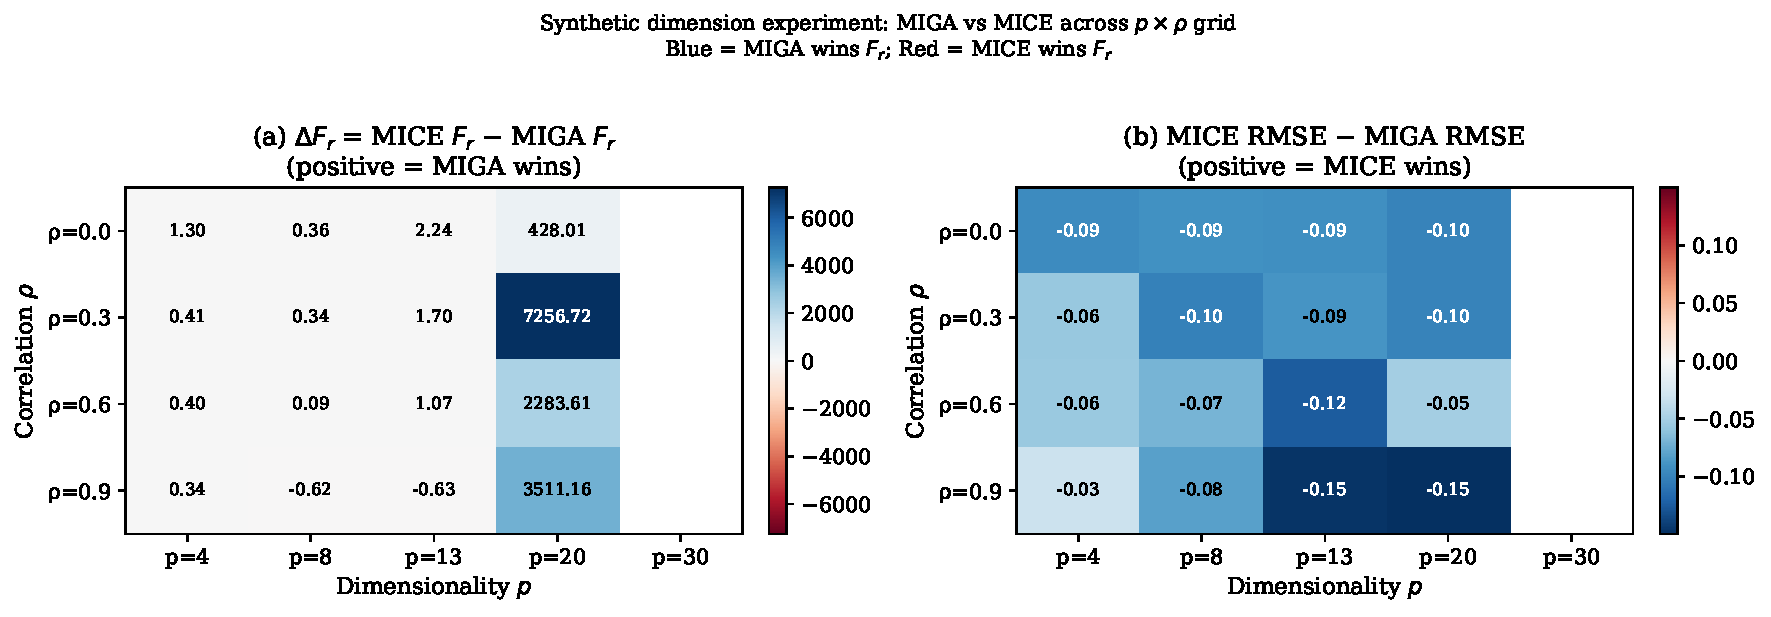
\includegraphics[width=0.85\textwidth]{Figures/fig5_synthetic_dim.pdf}
    \caption{Heatmap of MIGA's $F_r$ advantage ($\Delta F_r = F_r^{\text{MICE}} - \bar{F}_r^{\text{MIGA}}$) across the $p \times \rho$ grid. Green cells indicate MIGA achieves lower $F_r$ than MICE (positive advantage); red cells indicate MICE wins. Cells marked \dag\ (p=20) are degenerate due to near-zero complete rows; cells marked FAIL (p=30) indicate MIGA could not run (no complete rows available). The joint $(p,\rho)$ boundary is clearly visible: MIGA wins for $p \leq 13$ at $\rho \leq 0.6$ but loses at $\rho = 0.9$ even for $p = 8$.}
    \label{fig:synthetic_dim_design}
\end{figure}

%----------------------------------------------------------------------------------------

\section{Summary of Implementation Decisions}

\begin{table}[h]
\caption{Implementation decisions diverging from the paper specification.}
\label{tab:decisions}
\centering
\begin{tabular}{p{2.5cm}p{2.8cm}p{5.8cm}p{2.2cm}}
\toprule
\textbf{Decision} & \textbf{Paper spec.} & \textbf{Our implementation} & \textbf{Effect} \\
\midrule
Feature scaling       & Not mentioned  & Divide by $\hat{\sigma}_j$ from $X_A$ & Stabilises $d_{\text{cov}}$; required for Wine \\
Eigenvalue floor      & Not mentioned  & $\lambda_{\min} = \max(\lambda_{\max} \times 10^{-4}, 10^{-10})$ & Prevents division by zero \\
Generator type        & ``From samples'' & Bootstrap from observed values & Preserves discrete marginals \\
Covariance estimator  & Sample only    & Sample or Ledoit-Wolf (C2) & LW restores $d_{\text{cov}}=0$ at $n_A < p$ \\
Stopping criterion    & Not specified  & Budget-aware: early stop at stagnation $P=50$, restart within budget $B=Q \times G$ (C3) & More restarts, better landscape coverage \\
Diversity schedule    & Fixed 90\%     & Exponential decay $\alpha(g)=\exp(-\lambda g/G)$, $\lambda=2.0$ (C7) & Lower $F_r$, faster convergence \\
\bottomrule
\end{tabular}
\end{table}

%----------------------------------------------------------------------------------------

\section{Adaptive Diversity Injection --- AD-MIGA (C7)}
\label{sec:ad_miga_impl}

\subsection{Implementation}

The adaptive decay is implemented in \texttt{miga/core.py} via three new parameters:

\begin{itemize}
    \item \texttt{decay\_mode}: \texttt{'none'} (standard MIGA, fixed injection), \texttt{'linear'} (linear decay), or \texttt{'exponential'} (AD-MIGA-E)
    \item \texttt{decay\_lambda}: the exponential rate $\lambda$ (default 2.0)
    \item \texttt{diversity\_decay}: for linear decay, the fraction of reduction over $G$ generations (default 1.0 = full decay)
\end{itemize}

At each generation $g$, the number of diversity slots is computed as:

\begin{equation}
    n_{\text{div}}(g) = \max\!\left(0,\; \left\lfloor n_{\text{div}}^{\max} \cdot \exp\!\left(-\lambda \cdot \frac{g}{G}\right) \right\rfloor \right)
\end{equation}

where $n_{\text{div}}^{\max} = l - c - c_1 c_3 - 2(c_2 - 1)$ is the maximum diversity budget. Freed slots are reallocated to additional mutation offspring from the elite pool. The decay has no effect on the elite individuals or crossover offspring.

\subsection{Relationship to Budget-Aware Restarts (C3)}

AD-MIGA-E (exponential decay) is a within-run scheduling mechanism, while budget-aware restarts (C3) is a between-run scheduling mechanism. They are orthogonal and can be combined: an AD-MIGA run with early stopping would use less budget per run (allowing more restarts) while also improving each individual run's exploitation quality. This combination is identified as future work.

%----------------------------------------------------------------------------------------

\section{GAIN Implementation and \texorpdfstring{$\alpha$}{α}-Sweep Design (C8)}
\label{sec:gain_methods}

\subsection{Motivation}

Corollary~\ref{cor:gain_orthogonal} extends the $F_r$--RMSE orthogonality theorem to GAIN \cite{Yoon2018}. To test this empirically, we require a GAIN implementation that (i) shares no deep learning framework dependency with the rest of the codebase, (ii) is reproducible and seeded, and (iii) exposes the reconstruction weight $\alpha$ as a first-class parameter for the sweep.

\subsection{Pure NumPy GAIN Implementation}

We implement GAIN from scratch in NumPy (\texttt{miga/gain\_numpy.py}), avoiding any PyTorch or TensorFlow dependency. The implementation follows Yoon et al.\ (2018) exactly:

\begin{itemize}
    \item \textbf{Generator $G$}: 3-layer MLP with ReLU hidden activations and Sigmoid output. Input: $[\tilde{X}, M] \in \mathbb{R}^{2p}$ (data with missing replaced by noise, concatenated with mask). Output: imputed values $\hat{X} \in [0,1]^p$.
    \item \textbf{Discriminator $D$}: 3-layer MLP with the same architecture. Input: $[\hat{X}, H] \in \mathbb{R}^{2p}$ (reconstructed data with hint matrix). Output: per-feature probability of being observed.
    \item \textbf{Hint matrix $H$}: reveals a fraction \texttt{hint\_rate} $= 0.9$ of the true mask bits to $D$; remaining bits set to 0.5 (uninformative).
    \item \textbf{Optimiser}: Adam ($\eta = 10^{-3}$, $\beta_1 = 0.9$, $\beta_2 = 0.999$), implemented via manual backpropagation through each MLP.
\end{itemize}

The generator loss is:
\begin{equation}
    \mathcal{L}_G = \underbrace{\mathbb{E}[(1-M)\cdot\log D(\hat{X}, H)]}_{\text{adversarial}} + \alpha\underbrace{\mathbb{E}[M \cdot \|X - G(\tilde{X}, M)\|^2]}_{\text{MSE on observed}}
\end{equation}

where $\alpha > 0$ controls the balance between adversarial fidelity and reconstruction accuracy. All weights are initialised with He initialisation ($\sigma = \sqrt{2/\text{fan\_in}}$). Training runs for 5{,}000 iterations with batch size 128. Data are min-max normalised to $[0,1]$ before training and denormalised after imputation.

\subsection{\texorpdfstring{$\alpha$}{α}-Sweep Experimental Design}

To test whether any reconstruction weight places GAIN on the MIGA--MICE Pareto frontier, we sweep:
\begin{equation}
    \alpha \in \{0,\ 1,\ 10,\ 100,\ 1000,\ 10000\}
\end{equation}

with all other hyperparameters fixed. At $\alpha = 0$, GAIN is a pure adversarial imputer with no reconstruction signal. As $\alpha \to \infty$, the MSE term dominates and $G$ approaches a conditional mean estimator (MICE-like behaviour). For each $(\alpha, \text{dataset})$ pair, we run 5 independent seeds at 30\% MAR. MICE and MIGA (G=200, Q=2) are computed in the same loop as fixed reference anchors. Results are reported as $F_r$ vs RMSE trajectories, with each $\alpha$ value forming one point on the plane (Figures~\ref{fig:gain_alpha_traj}--\ref{fig:gain_alpha_lines}).

%----------------------------------------------------------------------------------------

\section{Parallel Execution of Independent GA Runs (C9)}
\label{sec:parallel_impl}

\subsection{Motivation}

MIGA's $Q$ independent GA runs are embarrassingly parallel: they share no state (no shared population, no shared fitness cache), and the final result is simply $\arg\min_{q} F_r^{(q)}$. At the thesis default Q=2, serial execution costs $\sim$200 seconds per seed. Reducing this is the primary practical obstacle to using MIGA in repeated-experiment settings.

\subsection{Implementation}

We add an \texttt{n\_jobs} parameter to \texttt{MIGA}:
\begin{itemize}
    \item \texttt{n\_jobs=1} — serial execution, identical to original behaviour
    \item \texttt{n\_jobs=N} — use $N$ worker processes
    \item \texttt{n\_jobs=-1} — use all available CPU cores
\end{itemize}

Parallelism is implemented via \texttt{concurrent.futures.ProcessPoolExecutor} (Python standard library, no additional dependencies). Each run executes in a subprocess via a module-level worker function \texttt{\_worker()}, which receives only picklable data across the process boundary: NumPy arrays (\texttt{X\_C\_base}, \texttt{col\_means}, \texttt{col\_stds}), the pre-computed \texttt{FitnessEvaluator} object, and scalar hyperparameters. Generator callables (which are lambda functions and therefore not picklable) are reconstructed inside each worker from \texttt{col\_means} and \texttt{col\_stds} using the worker's own RNG.

\subsection{Reproducibility Under Parallelism}

To ensure results are identical regardless of \texttt{n\_jobs}, we use \texttt{numpy.random.SeedSequence}:

\begin{enumerate}
    \item A master \texttt{SeedSequence} is constructed from the user-provided \texttt{seed}.
    \item $Q$ child sequences are spawned via \texttt{ss.spawn(Q)}, one per run.
    \item Each child sequence generates an integer seed passed to the subprocess.
    \item The subprocess constructs \texttt{np.random.default\_rng(child\_seed)}, independent of all other runs.
\end{enumerate}

This guarantees that Run $q$ always sees the same random stream regardless of whether the other $Q-1$ runs execute in the same process or separate ones. The $Q$ child seeds are deterministic functions of the master seed, so the full experiment is reproducible from a single integer.

\subsection{Benchmarks}

Table~\ref{tab:parallel_speedup} (Section~\ref{sec:future_neural} of Chapter~\ref{Chapter5}) reports wall-clock speedups across all 5 datasets at Q=2, G=200. Scaling is near-linear: 1.94--1.98$\times$, consistent across dimensionalities from $p=3$ (Haberman) to $p=13$ (Wine). The small gap from the theoretical 2.0$\times$ is subprocess startup and data serialisation overhead, which is fixed cost independent of $G$ and $l$.
